
\hkapitola{Objektové typy}

\kapitola{Struktury}

\begin{frame}[fragile]
\frametitle{Struktura -- struct}
\begin{bitemize}{struct}
\item \textbf{hodnotový typ} (předává se hodnota - nikoliv reference)
\item může obsahovat parametrické konstruktory, atributy, vlastnosti, metody, operátory, \ldots
\item nemůže definovat bezparametrický konstruktor, finalizér (destruktor)
\item \textbf{nemůže dědit} z předka
\begin{itemize}
\item vždy dědí z \lstinline|System.ValueType|, dědící z \lstinline|System.Object|
\end{itemize}
\item může realizovat \textbf{rozhraní}
\item instanci je možné vytvořit bez \lstinline|new|
\end{bitemize}
\end{frame}

\begin{frame}[fragile]
\frametitle{Struktura -- struct}
\begin{yesblock}
\begin{lstlisting}
struct Student
{
    public string FirstName;
    public string LastName;

    public Student(string firstName, string lastName)
    {
        FirstName = firstName;
        LastName = lastName;
    }
}
\end{lstlisting}
\end{yesblock}
\end{frame}

\begin{frame}[fragile]
\frametitle{Struktura -- struct}
\begin{yesblock}
\begin{lstlisting}[basicstyle=\small]
static void TestStudent()
{
    Student stPetraKratka = new Student("Petra", "Kratka");

    Student stJitkaMlada = new Student()
    {
        FirstName = "Jitka",
        LastName = "Mlada"
    };

    Student stPetrMaly = new Student();
    stPetrMaly.FirstName = "Petr";
    stPetrMaly.LastName = "Maly";

    Student stJanVelky; // pouze u struktur, nelze u tříd
    stJanVelky.FirstName = "Jan";
    stJanVelky.LastName = "Velky";
}
\end{lstlisting}
\end{yesblock}
\end{frame}


\kapitola{Třídy}

\begin{frame}[fragile]
\frametitle{Třídy -- class}
\begin{bitemize}{class}
\item \textbf{referenční typ} (předává se reference)
\item \textbf{jednoduchá dědičnost}
\begin{itemize}
\item může dědit z jednoho předka
\item rozlišuje se časná a pozdní vazba u metod
\end{itemize}
\item může realizovat \textbf{rozhraní}
\begin{itemize}
\item libovolný počet
\item implicitní/explicitní realizace rozhraní
\end{itemize}
\item může obsahovat konstruktory, finalizér, atributy, vlastnosti, události, metody, operátory, vnořené typy, \ldots
\item objekty jsou vytvářeny na haldě (heap)
\item paměť spravuje \textbf{garbage collector}
\end{bitemize}
\end{frame}



\begin{frame}[fragile]
\frametitle{Třídy -- porovnání s Javou/C++}
\begin{bitemize}{}
\item jednoduchá dědičnost
\begin{itemize}
\item logika dle javy, syntaxe dle C++
\end{itemize}
\item polymorfizmus
\begin{itemize}
\item v C++ je nutné řešit časnou/pozdní vazbu (\lstinline|virtual|), v C\# také (\lstinline|virtual, override|), Java toto zjednodušuje -- vše použije pozdní vazbu automaticky
\item systém v C\# je v zásadě složitější, umožňuje přerušit řetězec pozdní vazby \lstinline|new virtual|
\end{itemize}
\item rozhraní
\begin{itemize}
\item neřeší se viditelnost složek v rozhraní
\item dva způsoby realizace -- implicitní (standardní), explicitní (objekt je nutné přetypovat na typ rozhraní)
\end{itemize}
\end{bitemize}
\end{frame}



\begin{frame}[fragile]
\frametitle{Třídy -- porovnání s Javou/C++}
\begin{bitemize}{}
\item atributy a gettery/settery
\begin{itemize}
\item C\# zavádí pojem \textbf{vlastnost (property)} a speciální syntax nahrazující gettery, settery
\end{itemize}
\end{bitemize}
\end{frame}




\pkapitola{Třída -- Class}


\begin{frame}[fragile]
\frametitle{Třída -- class}
\vfill
\begin{noteblock}{}
\begin{lstlisting}
[viditelnost] [modifikátory] class NazevTridy [dědičnostARozhraní] { 
	[složkyTřídy]...
}
\end{lstlisting}
\end{noteblock}
\vfill
\begin{bitemize}{Viditelnost třídy}
\item \lstinline|internal| (výchozí) -- viditelná v rámci assembly
\item \lstinline|public| -- viditelná z ostatních assembly
\end{bitemize}
\vfill
\begin{bitemize}{Modifikátory}
\item \lstinline|abstract| -- abstraktní třída (nelze vytvořit instanci, obsahuje abstraktní složky)
\item \lstinline|static| -- statická třída (nelze vytvořit instanci, pouze statické složky)
\item \lstinline|sealed| -- zapečetěná třída (nelze z ní dědit)
\item \lstinline[morekeywords=partial]|partial| -- třída rozdělená do více souborů
\end{bitemize}
\vfill
\end{frame}




\begin{frame}[fragile]
\begin{bitemize}{Složky třídy}
\item konstruktory
\item konstanty
\item atributy
\item finalizéry
\item metody
\item vlastnosti
\item indexery
\item operátory
\item události
\item delegáty
\item třídy
\item rozhraní
\item struktury
\end{bitemize}
\end{frame}





\pkapitola{Objekty}




\begin{frame}[fragile]
\vfill
\begin{bitemize}{Objekt}
\item vytvořen pomocí \lstinline|new|
\item předáván referencí, paměť spravuje GC
\end{bitemize}
\vfill
\begin{yesblock}
\begin{lstlisting}
// nastavení reference na null
Osoba neexistujiciOsoba = null;

// volání bezparametrického konstruktoru
Osoba osobaVychozi = new Osoba();

// volání parametrického konstruktoru
Osoba osobaParametricka = new Osoba("Franta", "Maly");
\end{lstlisting}
\end{yesblock}
\vfill
\end{frame}



\begin{frame}[fragile]
\vfill
\begin{bitemize}{}
\item C\# umožňuje kombinovat volání konstruktoru a inicializaci vlastností
\end{bitemize}
\vfill
\begin{yesblock}
\begin{lstlisting}
Osoba osobaZvlastni = new Osoba() {
	Jmeno = "Franta",
	Prijmeni = "Maly"
};

// uvedený kód je ekvivalentem:
Osoba osobaZvlastni = new Osoba();
osobaZvlastni.Jmeno = "Franta";
osobaZvlastni.Prijmeni = "Maly";
\end{lstlisting}
\end{yesblock}
\vfill
\end{frame}



\begin{frame}[fragile]
\vfill
\begin{bitemize}{Objekt -- porovnávání}
\item \lstinline|==, Equals| -- porovnání referencí/obsahu (nezávisle přetížitelné)
\item \lstinline|object.ReferenceEquals()| -- vždy porovná shodu referencí
\end{bitemize}
\vfill
\begin{yesblock}
\begin{lstlisting}[basicstyle=\small]
Osoba mojeOsoba = new Osoba();
Osoba ciziOsoba = mojeOsoba;

//var wl = (Action<string>)Console.WriteLine;
wl($"==: {mojeOsoba == ciziOsoba}");
wl($"Equals: {mojeOsoba.Equals(ciziOsoba)}");
wl($"ReferenceEquals: {object.ReferenceEquals(mojeOsoba, ciziOsoba)}");
// True, True, True

ciziOsoba = new Osoba();

wl($"==: {mojeOsoba == ciziOsoba}");
wl($"Equals: {mojeOsoba.Equals(ciziOsoba)}");
wl($"ReferenceEquals: {object.ReferenceEquals(mojeOsoba, ciziOsoba)}");
// True/False, True/False, False
\end{lstlisting}
\end{yesblock}
\vfill
\end{frame}




\begin{frame}[fragile]
\begin{bonusblock}{Ukázka přetěžování Equals a operátorů ==, !=}
\begin{lstlisting}[basicstyle=\small]
class Osoba
{
	public string Jmeno { get; set; }
	public string Prijmeni { get; set; }
	
	public override bool Equals(object obj)
	{
	    if (obj == null || GetType() != obj.GetType())
	        return false;
	
	    Osoba osoba = (Osoba)obj;
	    return Jmeno == osoba.Jmeno && Prijmeni == osoba.Prijmeni;
	}
	
	public override int GetHashCode()
	{
		return 11 * Jmeno.GetHashCode() + Prijmeni.GetHashCode();
	}
\end{lstlisting}
\end{bonusblock}
\end{frame}


\begin{frame}[fragile]
\vfill
\begin{bonusblock}{~}
\begin{lstlisting}[basicstyle=\small]
	public static bool operator ==(Osoba osa, Osoba osb)
	{
	    return osa.Equals(osb);
	}
	
	public static bool operator !=(Osoba osa, Osoba osb)
	{
	    return !(osa == osb);
	}
}
\end{lstlisting}
\end{bonusblock}
\vfill
\begin{bitemize}{Přetěžování Equals, ==, !=}
\item pokud to má smysl přetižte \lstinline|Equals| (a \lstinline|GetHashCode|) u hodnotových i referenčních typů
\item přetižte ==
\begin{itemize}
\item pokud se jedná o hodnový typ
\item pokud se jedná o referenční \uv{základní} typ (\lstinline|Point|, \lstinline|string|, \lstinline|BigNumber|) nebo pokud přetěžujete operátory +, -, \ldots
\end{itemize}
\end{bitemize}
\vfill
\end{frame}



\begin{frame}[fragile]
\begin{bitemize}{Vnořené třídy a struktury}
\item třída může obsahovat vnořené třídy a struktury
\item mezi nadřazenou a vnořenou třídou neexistuje žádné spojení
\begin{itemize}
\item chování odpovídá v Javě vnořené třídě definované jako statické
\item stejné chování mají vnořené typy v C++
\end{itemize}

\item ve vnořených typech se, ale uplatňuje genericita nadřazeného prvku
\item objekt vnořeného typ se vytváří pomocí nadřazeného typu, nikoliv instance
\begin{itemize}
\item \lstinline|Outer.Inner instance = new Outer.Inner(...);|
\end{itemize}

\end{bitemize}
\vfill
\begin{noblock}
\begin{lstlisting}
class Outer { private int i; class Inner { ...  } }

// Inner::method
void Method() {
  // všechny zápisy jsou neplatné - neexistuje spojení mezi objekty
  Outer.this.i = 0;
  Outer.i = 0;
  i = 0;
}
\end{lstlisting}
\end{noblock}
\end{frame}




\kapitola{Složky třídy}




\begin{frame}[fragile]
\begin{bitemize}{Viditelnost složek}
\item \lstinline|public| -- veřejná (všude)
\item \lstinline|private| -- privátní (pouze definující třída), výchozí pro složky tříd a struktur
\item \lstinline|protected| -- chráněná (třída nebo její potomci)
\item \lstinline|internal| -- interní (assembly)
\item \lstinline|protected internal| -- sjednocení \lstinline|protected| a \lstinline|internal| (assembly a potomci (i z jiného assembly))
\item \lstinline|private protected| -- \lstinline|protected|, ale pouze u potomků ve stejném assembly
\end{bitemize}
\end{frame}






\pkapitola{Konstruktory, finalizér}



\begin{frame}[fragile]
\frametitle{Konstruktory}
\vfill
\begin{noteblock}{}
\begin{lstlisting}
[viditelnost] [modifikátory] NázevTřídy([parametry]) [voláníJinéhoKonstruktoru]
\end{lstlisting}
\end{noteblock}
\vfill
\begin{yesblock}
\begin{lstlisting}[basicstyle=\small]
class Student
{
    // Bezparametrický konstruktor - volá se při new Student()
    public Student() { }

    // Parametrický konstruktor - volá se při new Student(string, string)
    public Student(string jmeno, string prijmeni) { }

    // Statický konstruktor - volá se při zavedení typu do paměti
    static Student() { }
}
\end{lstlisting}
\end{yesblock}
\vfill
\end{frame}


\begin{frame}[fragile]
\frametitle{Finalizéry}
\vfill
\begin{noteblock}{}
\begin{lstlisting}
~NázevTřídy() { ... }
\end{lstlisting}
\end{noteblock}
\vfill
\begin{bitemize}{}
\item slouží k uvolnění prostředů
\item implicitně volá metodu \lstinline|object.Finalize|
\item používán spíše výjimečně, není zaručeno, kdy dojde k jeho zavolání
\item pro řízené uvolnění prostředků existuje rozhraní \lstinline|IDisposable|
\end{bitemize}
\vfill
\begin{yesblock}
\begin{lstlisting}
public class Auto 
{
    ~Auto() 
    {
        // ...
    }
}
\end{lstlisting}
\end{yesblock}
\vfill
\end{frame}






\pkapitola{Atributy, vlastnosti}


\begin{frame}[fragile]
\begin{bitemize}{}
\item Atribut (Attribute) -- Java, C++, C\#
\begin{itemize}
\item má identifikátor, datový typ, přístupová práva
\item alokuje místo v paměti pro uložení hodnoty datového typu (představuje datovou složku)
\item \lstinline|private string name;|
\end{itemize}
\vskip 2ex
\item Vlastnost (Property) -- C\#
\begin{itemize}
\item má identifikátor, datový typ, přístupová práva
\item definuje getter a setter, jak přistoupit k datové složce
\item není atributem, neobsahuje data!
\item \lstinline|public string Name { get { return name;} set { name = value; } }|
\end{itemize}
\end{bitemize}
\end{frame}



\begin{frame}[fragile]
\frametitle{Atributy (datové složky)}
\vfill
\begin{noteblock}{}
\begin{lstlisting}
[viditelnost] [modifikátory] datovýTyp názevAtributu [inicializér];
\end{lstlisting}
\end{noteblock}
\vfill
\begin{bitemize}{Modifikátor}
\item \lstinline|static| -- statická složka (neváže se na instanci)
\item \lstinline|const| -- konstanta, musí být nastavena v inicializéru
\item \lstinline|readonly| -- konstanta, musí být nastavena v konstruktoru
\end{bitemize}
\vfill
\end{frame}



\begin{frame}[fragile]
\frametitle{Statické složky (atributy, metody)}
\vfill
\begin{yesblock}
\begin{lstlisting}
class Osoba
{
    public static int PocetInstanci;

    public Osoba() 
    { 
        PocetInstanci++; 
    }
}
\end{lstlisting}
\end{yesblock}
\vfill
\begin{yesblock}
\begin{lstlisting}
int pocet = Osoba.PocetInstanci;
\end{lstlisting}
\end{yesblock}
\vfill
\end{frame}



\begin{frame}[fragile]
\frametitle{Statická třída}
\vfill
\begin{yesblock}
\begin{lstlisting}
static class Matematika
{
    public const double Pi = 3.141592;

    public static double Odmocnina(double hodnota)
    {
        return Math.Sqrt(hodnota);
    }
}
\end{lstlisting}
\end{yesblock}
\vfill
\begin{yesblock}
\begin{lstlisting}
double pi = Matematika.Pi;
double sqrt = Matematika.Odmocnina(72);
\end{lstlisting}
\end{yesblock}
\vfill
\begin{noblock}
\begin{lstlisting}
Matematika matematika = new Matematika();
\end{lstlisting}
\end{noblock}
\vfill
\end{frame}






\begin{frame}[fragile]
\frametitle{const/readonly složky}
\vfill
\begin{yesblock}
\begin{lstlisting}
class IdGenerator
{
    const int prvniId = 123;
    readonly string prefixId;

    public IdGenerator(string prefix)
    {
        // const nelze inicializovat v konstruktoru
        // prvniId = 100;

        // readonly musí být inicializován v konstruktoru
        prefixId = prefix;
    }
}
\end{lstlisting}
\end{yesblock}
\vfill
\end{frame}



\pkapitola{Vlastnost -- Property}


\begin{frame}[fragile]
\frametitle{Vlastnosti}
\vfill
\begin{bitemize}{}
\item definují getter a setter pro přístup k datové složce
\item obyčejná vlastnost neobsahuje data
\item uvnitř setteru je nastavovaná hodnota předána skrze klíčové slovo \lstinline|value|
\end{bitemize}
\vfill
\begin{yesblock}
\begin{lstlisting}[morekeywords=value]
class Student
{
    // atribut - uchovává hodnotu
    private string firstName; 
    // vlastnost - definuje pravidla pro přístup k atributu
    public string FirstName 
    {
        get { return firstName; }
        set { firstName = value; }
    }
}
\end{lstlisting}
\end{yesblock}
\vfill
\end{frame}



\begin{frame}[fragile]
\frametitle{Vlastnosti}
\begin{yesblock}
\begin{lstlisting}[morekeywords=value]
class Student
{
    private string netID;
    public string NetID
    {
        get { return netID; }
        set
        {
            if (value.StartsWith("st") && value.Length == 7)
                netID = value;
        }
    }
}
\end{lstlisting}
\end{yesblock}
\end{frame}


\begin{frame}[fragile]
\frametitle{Vlastnosti -- zkrácený zápis}
\vfill
\begin{bitemize}{C\# 7}
\item tělo metody/getteru/setteru lze zkrátit na výraz pomocí \textbf{=>}
\end{bitemize}
\vfill
\begin{yesblock}
\begin{lstlisting}[morekeywords=value]
private string firstName;
public string FirstName
{
    get => firstName;
    set => firstName = value;
}
\end{lstlisting}
\end{yesblock}
\vfill
\end{frame}


\begin{frame}[fragile]
\frametitle{Vlastnosti -- viditelnost}
\vfill
\begin{bitemize}{}
\item lze definovat viditelnost operací
\begin{itemize}
\item pokud není uvedena u konkrétní operace, použije se viditelnost uvedená u vlastnosti
\end{itemize}

\end{bitemize}
\vfill
\begin{yesblock}
\begin{lstlisting}[morekeywords=value]
private string firstName;
public string FirstName
{
    private get => firstName;
    protected set => firstName = value;
}
\end{lstlisting}
\end{yesblock}
\vfill
\end{frame}


\begin{frame}[fragile]
\frametitle{Vlastnosti -- pouze setter/getter}
\vfill
\begin{bitemize}{}
\item lze definovat pouze setter/getter
\end{bitemize}
\vfill
\begin{yesblock}
\begin{lstlisting}
private List<Student> studenti;
public int PocetStudentu
{
    get => studenti.Count;
}
\end{lstlisting}
\end{yesblock}
\vfill
\end{frame}


\begin{frame}[fragile]
\frametitle{Vlastnosti -- automaticky implementované vlastnosti}
\vfill
\begin{bitemize}{}
\item kompilátor na pozadí vytvoří atribut pro uložení hodnoty
\item atribut (datová složka) je neviditelná a není přímo přístupná
\item není možné upravit chování \lstinline|get| nebo \lstinline|set| operace, lze upravit viditelnost
\end{bitemize}
\vfill
\begin{yesblock}
\begin{lstlisting}
public string FirstName { get; set; }
public string MiddleName { get; set; }
public string LastName { get; set; }

// od C# 6 - lze automaticky impl. vlastnosti rovnou inicializovat
public string NetID { get; set; } = "st12345";
// od C# 6 - lze definovat read-only auto prop. s inicializací v konstruktoru
public uint StudentID { get; }
//// konstruktor
//// StudentID = 12345;
\end{lstlisting}
\end{yesblock}
\vfill
\end{frame}



\begin{frame}[fragile]
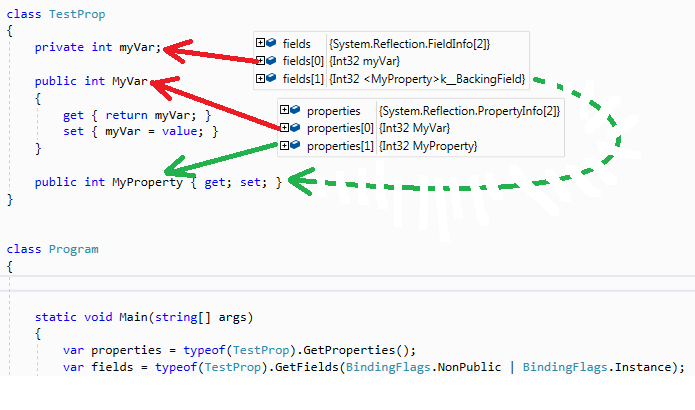
\includegraphics[width=\textwidth]{img/property_backing_field.png}
\end{frame}



\begin{frame}[fragile]
\frametitle{Javism -- gettery a settery}
\vfill
\begin{noblock}
\begin{lstlisting}[basicstyle=\small]
// String - klíčové slovo "string"
// atribut - místo vlastnosti
private String name;

// metoda jako getter a setter místo vlastosti
public String getName() {
    return name;
}

public void setName(String name) {
    this.name = name;
}
\end{lstlisting}
\end{noblock}
\vfill
\begin{yesblock}
\begin{lstlisting}[basicstyle=\small]
// "string"
// veřejná vlastnost - začíná velkým písmenem
public string Name { get; set; }
\end{lstlisting}
\end{yesblock}
\vfill
\end{frame}


\begin{frame}[fragile]
\begin{bitemize}{Vytváření vlastností ve Visual Studiu}
\item vlastnosti lze velmi efektivně vytvářet pomocí připravených code-snippets
\item []
\item \lstinline|prop<TAB><TAB>| -- vytvoří automaticky implementovanou vlastnost (TAB - přepíná mezi jednotlivými editovatelnými částmi)
\item \lstinline|propg<TAB><TAB>| -- stejné jako předchozí, ale je nastaveno \lstinline|private set|
\item \lstinline|propfull<TAB><TAB>| -- vytvoří vlastnost a backing atribut pro ní
\item \lstinline|propdp<TAB><TAB>| -- dependency property
\item \lstinline|propa<TAB><TAB>| -- attached dependency property
\end{bitemize}
\end{frame}


\kapitola{Metody}


\begin{frame}[fragile]
\frametitle{Metody}
\vfill
\begin{noteblock}{}
\begin{lstlisting}
[viditelnost] [modifikátory] typNávratovéHodnoty názevMetody([parametry]) těloMetody

těloMetody:
	=> výraz
	{ [příkazy] }
\end{lstlisting}
\end{noteblock}
\vfill
\begin{bitemize}{Modifikátory}
\item \lstinline|static| -- statická metoda
\item \lstinline|new| -- zakrývání metody z předka
\item \lstinline|virtual| -- virtuální metoda (polymorfizmus)
\item \lstinline|override| -- přetížená metoda (polymorfizmus)
\item \lstinline|abstract| -- abstraktní metoda (polymorfizmus)
\item \lstinline[morekeywords=async]|async| -- asynchronní metody
\end{bitemize}
\vfill
\end{frame}



\begin{frame}[fragile]
\frametitle{Metody -- příklad}
\vfill
\begin{yesblock}
\begin{lstlisting}[basicstyle=\small]
class Student
{
    public string Name { get; set; }

    public void SayHello()
    {
        Console.WriteLine($"Hello, I'm {Name}");
    }
}
\end{lstlisting}
\end{yesblock}
\vfill
\begin{yesblock}
\begin{lstlisting}[basicstyle=\small]
Student peter = new Student()
{
    Name = "Peter"
};

peter.SayHello();
\end{lstlisting}
\end{yesblock}
\vfill
\end{frame}




\begin{frame}[fragile]
\frametitle{Metody -- příklad zkráceného zápisu}
\vfill
\begin{yesblock}
\begin{lstlisting}[basicstyle=\small]
class Student
{
    public string Name { get; set; }

    public void SayHello() => Console.WriteLine($"Hello, I'm{Name}");
}
\end{lstlisting}
\end{yesblock}
\vfill
\end{frame}




\begin{frame}[fragile]
\frametitle{Metody -- výchozí hodnota parametru}
\begin{bitemize}{}
\item parametry mohou mít uvedenou výchozí hodnotu
\end{bitemize}
\vfill
\begin{yesblock}
\begin{lstlisting}[basicstyle=\small]
class MyMath
{
    public const double Pi = 3.141592;

    public static double GetPowerOfPi(int power = 1)
    {
        return Math.Pow(Pi, power);
    }
}
\end{lstlisting}
\end{yesblock}
\vfill
\begin{yesblock}
\begin{lstlisting}[basicstyle=\small]
double pi = MyMath.GetPowerOfPi();
double piSquare = MyMath.GetPowerOfPi(2);
\end{lstlisting}
\end{yesblock}
\end{frame}




\begin{frame}[fragile]
\frametitle{Metody -- ref}
\begin{bitemize}{}
\item parametr je možné předat odkazem (referencí)
\begin{itemize}
\item u parametru i u hodnoty argumentu je nutné uvést \lstinline|ref|
\end{itemize}

\end{bitemize}
\vfill
\begin{yesblock}
\begin{lstlisting}[basicstyle=\small]
class Toolkit
{
    public static void Increment(ref int value)
    {
        value++;
    }
}
\end{lstlisting}
\end{yesblock}
\vfill
\begin{yesblock}
\begin{lstlisting}[basicstyle=\small]
int intValue = 0;
Toolkit.Increment(ref intValue);
Console.WriteLine($"{intValue}");
\end{lstlisting}
\end{yesblock}
\end{frame}



\begin{frame}[fragile]
\frametitle{Metody -- out}
\begin{bitemize}{}
\item parametr může být výstupní
\begin{itemize}
\item u parametru i u hodnoty argumentu je nutné uvést \lstinline|out|
\end{itemize}

\end{bitemize}
\vfill
\begin{yesblock}
\begin{lstlisting}[basicstyle=\small]
class AuthenticationService
{
    public static bool Authentize(string password, out string username)
    {
        if (password == "secr3tP4ssw0rd!")
        {
            username = "admin";
            return true;
        }

        username = null;
        return false;
    }
}
\end{lstlisting}
\end{yesblock}
\end{frame}

\begin{frame}[fragile]
\frametitle{Metody -- out}
\vfill
\begin{yesblock}
\begin{lstlisting}[basicstyle=\small]
string username;
if(AuthenticationService.Authentize("password", out username))
{
    Console.WriteLine($"Authenticated as {username}");
}
\end{lstlisting}
\end{yesblock}
\vfill
\begin{yesblock}
\begin{lstlisting}[basicstyle=\small]
// C# 7 - podporuje deklarovat proměnnou v místě volání
if(AuthenticationService.Authentize("password", out string username))
{
    Console.WriteLine($"Authenticated as {username}");
}
\end{lstlisting}
\end{yesblock}
\vfill
\end{frame}




\nezkouskove

\begin{frame}[fragile]
\frametitle{Metody -- params}
\begin{bitemize}{}
\item je možné volat metodu s libovolným počtem parametrů (stejného typu)
\begin{itemize}
\item předáváno jako parametr typu pole s mod. \lstinline|params|
\item \lstinline|params| parametr musí být uveden jako poslední v seznamu parametrů
\end{itemize}

\end{bitemize}
\vfill
\begin{yesblock}
\begin{lstlisting}[basicstyle=\small]
public static int SumArguments(params int[] arguments)
{
    int sum = 0;
    foreach (var item in arguments)
    {
        sum += item;
    }

    return sum;
}
\end{lstlisting}
\end{yesblock}
\vfill
\begin{yesblock}
\begin{lstlisting}[basicstyle=\small]
int result = Summer.SumArguments(10, 20, 30, 40, 50, 60, 70);
\end{lstlisting}
\end{yesblock}
\end{frame}





\begin{frame}[fragile]
\frametitle{Metody -- pojmenované argumenty}
\begin{bitemize}{}
\item při volání metody je možné specifikovat argumenty v libovolném pořadí, pokud je uveden jejich název
\begin{itemize}
\item zapisuje se jako: \lstinline|názevParametru: hodnota|
\end{itemize}

\end{bitemize}
\vfill
\begin{yesblock}
\begin{lstlisting}[basicstyle=\small]
public static void AddProduct(string productName, int count = 1, 
    double weight = 0, string description = "")
\end{lstlisting}
\end{yesblock}
\vfill
\begin{yesblock}
\begin{lstlisting}[basicstyle=\small]
AddProduct("Toy", 10, 1.2, "Kid's toy");
AddProduct("Toy", count: 10, weight: 1.2);
AddProduct("Toy", description: "Kid's toy", count: 10);
// od C# 7.2:
AddProduct(productName: "Toy", 10, description: "Kid's toy"); 
\end{lstlisting}
\end{yesblock}
\end{frame}




\begin{frame}[fragile]
\frametitle{Metody -- ref return}

\begin{bitemize}{}
\item z metody je možné vracet referenci (C\# 7, mod. \lstinline|ref|)
\end{bitemize}
\vfill
\begin{yesblock}
\begin{lstlisting}[basicstyle=\small]
public static ref int FindGreaterThan(int[] array, int condition)
{
    for (int i = 0; i < array.Length; i++)
        if (array[i] > condition)
            return ref array[i];

    throw new Exception("Not found");
}
\end{lstlisting}
\end{yesblock}
\vfill
\begin{yesblock}
\begin{lstlisting}[basicstyle=\small]
int[] array = { 1, 2, 5, 15, 32, 64 };
Console.WriteLine($"{string.Join(" ", array)}");
ref int value = ref FindGreaterThan(array, 10);
value += 100;
Console.WriteLine($"{string.Join(" ", array)}");
\end{lstlisting}
\end{yesblock}
\end{frame}





\begin{frame}[fragile]
\frametitle{Metody -- rozšiřující (extension) metody}

\begin{bitemize}{}
\item (statická) metoda se tváří jako (instanční) metoda jiné třídy
\begin{itemize}
\item rozšířená třída je uvedena jako první parametr metody s mod. \lstinline|this|
\item metoda se volá přímo nad objektem rozšířené třídy
\end{itemize}

\item poprvé masivně použito pro realizaci LINQ
\end{bitemize}
\vfill
\begin{yesblock}
\begin{lstlisting}[basicstyle=\small]
class Student
{
  public string Name { get; set; }
}

static class StudentExtension
{
  public static void SayHello(this Student student, string weather)
  {
    Console.WriteLine($"Hello, I'm {student.Name} and it's {weather}");
  }
}
\end{lstlisting}
\end{yesblock}
\end{frame}

\begin{frame}[fragile]
\frametitle{Metody -- rozšiřující (extension) metody}
\begin{yesblock}
\begin{lstlisting}[basicstyle=\small]
Student student = new Student()
{
    Name = "Peter"
};

student.SayHello("sunny");
//Hello, I'm Peter and it's sunny
\end{lstlisting}
\end{yesblock}
\end{frame}


\zkouskove